\documentclass[review]{elsarticle}
% for submission use preprint
% review for

\usepackage{lineno,hyperref}
\usepackage{amsmath}
\modulolinenumbers[5]

\journal{Journal of Networks and Computer Applications}

%%%%%%%%%%%%%%%%%%%%%%%
%% Elsevier bibliography styles
%%%%%%%%%%%%%%%%%%%%%%%
%% To change the style, put a % in front of the second line of the current style and
%% remove the % from the second line of the style you would like to use.
%%%%%%%%%%%%%%%%%%%%%%%

%% Numbered
%\bibliographystyle{model1-num-names}

%% Numbered without titles
%\bibliographystyle{model1a-num-names}

%% Harvard
%\bibliographystyle{model2-names.bst}\biboptions{authoryear}

%% Vancouver numbered
%\usepackage{numcompress}\bibliographystyle{model3-num-names}

%% Vancouver name/year
%\usepackage{numcompress}\bibliographystyle{model4-names}\biboptions{authoryear}

%% APA style
%\bibliographystyle{model5-names}\biboptions{authoryear}

%% AMA style
%\usepackage{numcompress}\bibliographystyle{model6-num-names}

%% `Elsevier LaTeX' style
\bibliographystyle{elsarticle-num}
%%%%%%%%%%%%%%%%%%%%%%%

\begin{document}

\begin{frontmatter}

\title{A wearable fall-detection system based on Body Area Networks for smart cities}

%% Group authors per affiliation:
\author{Luigi La Blunda\fnref{label1}}
\ead{l.lablunda@fb2.fra-uas.de (corresponding author)}
\author{Lorena Guti\'errez-Madro\~nal\fnref{label2}}
%% \author{Name\corref{cor1}\fnref{label2}}
\ead{lorena.gutierrez@uca.es}
\author{Matthias F. Wagner\fnref{label1}}
\ead{mfwagner@fb2.fra-uas.de}
\author{I. Medina-Bulo\fnref{label2}}
\ead{inmaculada.medina@uca.es}
\address[label1]{WSN and IOT Research Group Frankfurt University of Applied Sciences, Nibelungenplatz 1, 60318 Frankfurt am Main, Germany}
\address[label2]{UCASE Software Engineering Research group, University of Cadiz}



%% or include affiliations in footnotes:
%\author[mymainaddress,mysecondaryaddress]{Elsevier Inc}
%\ead[url]{www.elsevier.com}
%
%\author[mysecondaryaddress]{Global Customer Service\corref{mycorrespondingauthor}}
%\cortext[mycorrespondingauthor]{Corresponding author}
%\ead{support@elsevier.com}
%
%\address[mymainaddress]{1600 John F Kennedy Boulevard, Philadelphia}
%\address[mysecondaryaddress]{360 Park Avenue South, New York}

\begin{abstract}
Falls can have serious consequences for people, which can lead, for example, to restrictions in mobility or in the worst case to traumatic based cases of death. To provide rapid assistance, a portable fall detection system has been developed which is capable of detecting fall situations and, if necessary, alerting the emergency services without any user interaction. The prototype was designed to facilitate a reliable fall-detection and to classify several fall-types. This solution represents a life-saving service for every inhabitant which would significantly enrich the development of smart cities and smart factories where fall-events are part of daily-life. This paper will also introduce the fall analysis, which includes the generation of test events. To guarantee functional safety, the hazard analysis method STAMP (System-Theroetic Accident Model and Processes) will be applied. 
\end{abstract}

\begin{keyword}
e-Health \sep fall-detection\sep Body Area Network \sep safety \sep STAMP \sep Smart City \ 
\end{keyword}

\end{frontmatter}

%\linenumbers

\section{Introduction}
Fall-detection is gaining in importance not only in aging societies, but also in working society and in daily activities. According to the World Health Organization (WHO), 646,000 fatal falls are estimated to be the second leading cause of accidental or unintentional death worldwide each year. People over 65 suffer the most fatal falls. Another high risk group is children. Taking into consideration their evolving developmental stages, the increasing curiosity to explore the environment or the inadequate adult supervision lead to fall-events \cite{WHO2018}.
In everyday life we are also confronted with risk of falling. Working in hazardous working conditions is another risk factor for causing fall-events. An exemplary event could be a worker that falls during the night shift in the factory and no one is there to provide prompt assistance. Another example could be a technician which falls from height while maintaining windmills. Mostly windmills are installed in uninhabited areas where no immediate rescue measures can be taken. Considering these events the consequences can be fatal for the affected people. 
The World Health Organization stated that annually 37.3 million fall-events are severe enough to require medical treatment \cite{WHO2018}. Fall-events leads to the side effects of physical inactivity and loss of balance, especially among old people. Elderly people are scared to fall again and this uncertainty of movement increases the risk of repeated falls. 
To counteract these life-threatening events fast assistance is necessary due to the fact that an unconscious person may not be able to call the emergency services. An approach could be the continuous tracing of medical and / or physical parameters via a wearable sensor network (see Figure \ref{fig:escalationscheme}).
\begin{figure}[!ht]
	\centering
	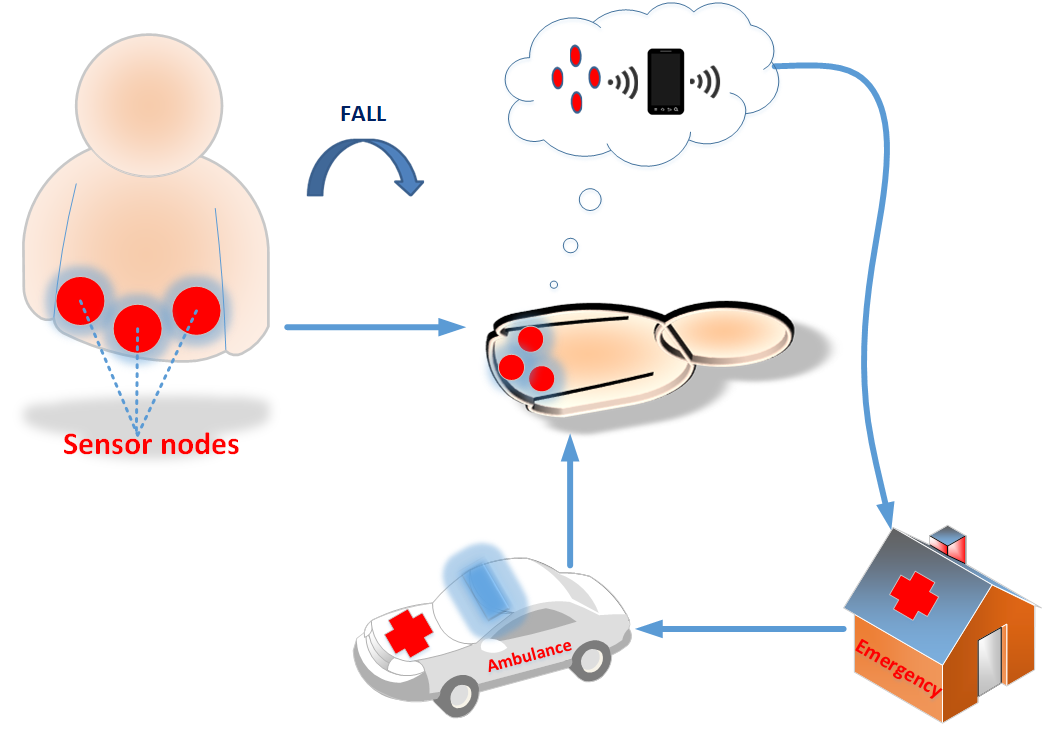
\includegraphics[scale=0.35]{Images/EscalationScheme}
	\caption[Escalation scheme]{Escalation scheme simulation~\cite{LaBlunda.2016,LaBlunda.2016b}}
	\label{fig:escalationscheme}
\end{figure}
A prototype in form of a belt was developed which includes an Electrocardiogram (ECG) - harness and is based on a five sensor nodes Body Area Network (BAN). Each sensor node of the belt acquires continuously acceleration data including time stamp and the sensor node of the ECG-harness provides the analog value of the voltage including time stamp. In case of a fall the system should be capable to autonomously call the emergency services. Applying sensor fusion of physical and medical sensors we expect to improve the reliability of fall-detection and possibly fall-prevention. Another expectation is that the integration of medical sensors may facilitate the classification of different fall-types. In terms of smart cities our expectancy is to significantly provide an important e-health service for smart cities which is an essential life-saver for the population.

The paper is structured as follows. Section \ref{sec:relatedwork} describes the related work regarding fall-detection. In this section a short overview about existing solutions and different approaches for fall-detection is given. Section \ref{sec:background} will describe the basic principles on which our ongoing fall-detection research is based. In the successive section (Section \ref{sec:fall-detectionPrototype}) a detailed description of the fall-detection prototype, including the usage of sensor are introduced. Additionally, this section contains the generation of test events which includes the results of the fall-analysis and detected problems. Section \ref{sec:STAMP} will introduce the Hazard analysis method STAMP which is applied on the fall-detection prototype.
Finally, in section \ref{sec:conclusion} a conclusion about this ongoing research is given, including some indications for improvement which could be applied in the future work.

\section{Related Work}
\label{sec:relatedwork}
In this section an overview about several fall-detection approaches is given. There are several techniques which can be applied to detect fall-events. Igual et al. \cite{Igual2013} illustrates the following different types of fall-detection  systems:
\begin{itemize}
	\item Context-aware systems
	\item Wearable systems
\end{itemize}
The functionality of context-aware systems depends on the environment, since the sensors and actuators must be installed in the living area (apartment, nursing home) in order to detect possible fall situations. The video-based context-aware solutions have the advantage to provide an accurate and reliable detection of falls with a fast assistance, but these systems have an issue regarding privacy. Patients using this solution are non-stop monitored and this is not well accepted by many. Additionally, the high purchase price is an obstacle for many patients and the dependency on the environment makes this approach useless, because it would not detect fall-events happening outside the networked area.

The other category of fall-detection systems analyzed by Igual et al. \cite{Igual2013} contains wearable solutions worn on the body and are based on Body Area Networks (BAN). This solution is capable to provide a fall-detection which is independent from the environment in contrast to context-aware systems. The analysis of Igual et al. \cite{Igual2013} illustrates wearable fall-detection systems using the sensor fusion method which comprises accelerometer and gyroscope data and built-in systems in form of smart phone sensors. For both categories of fall-detection solutions (context-aware \& wearable solution) several techniques were used. The following methods were applied for context-aware systems:
\begin{itemize}
	\item Image processing and threshold-based recognition
	\item Image processing and classification models
\end{itemize}
The techniques used for the fall-detection in wearable solutions are the following:
\begin{itemize}
	\item Threshold-based approach
	\item Fall-detection based on machine learning
\end{itemize}
Taking into consideration the fact that it is an essential advantage to focus on wearable solution because of the system's functional independence the scientific work of Li et al. \cite{Li2009} will be explained subsequently. The solution of Li et al. \cite{Li2009} includes two wearable sensor nodes which are based on a BAN. These sensor nodes consist of an accelerometer and gyroscope and they are placed on the chest (Node A) and on the thigh (Node B, see Figure \ref{fig:LietAl-Architecture}). 
\begin{figure}[!ht]
	\centering
	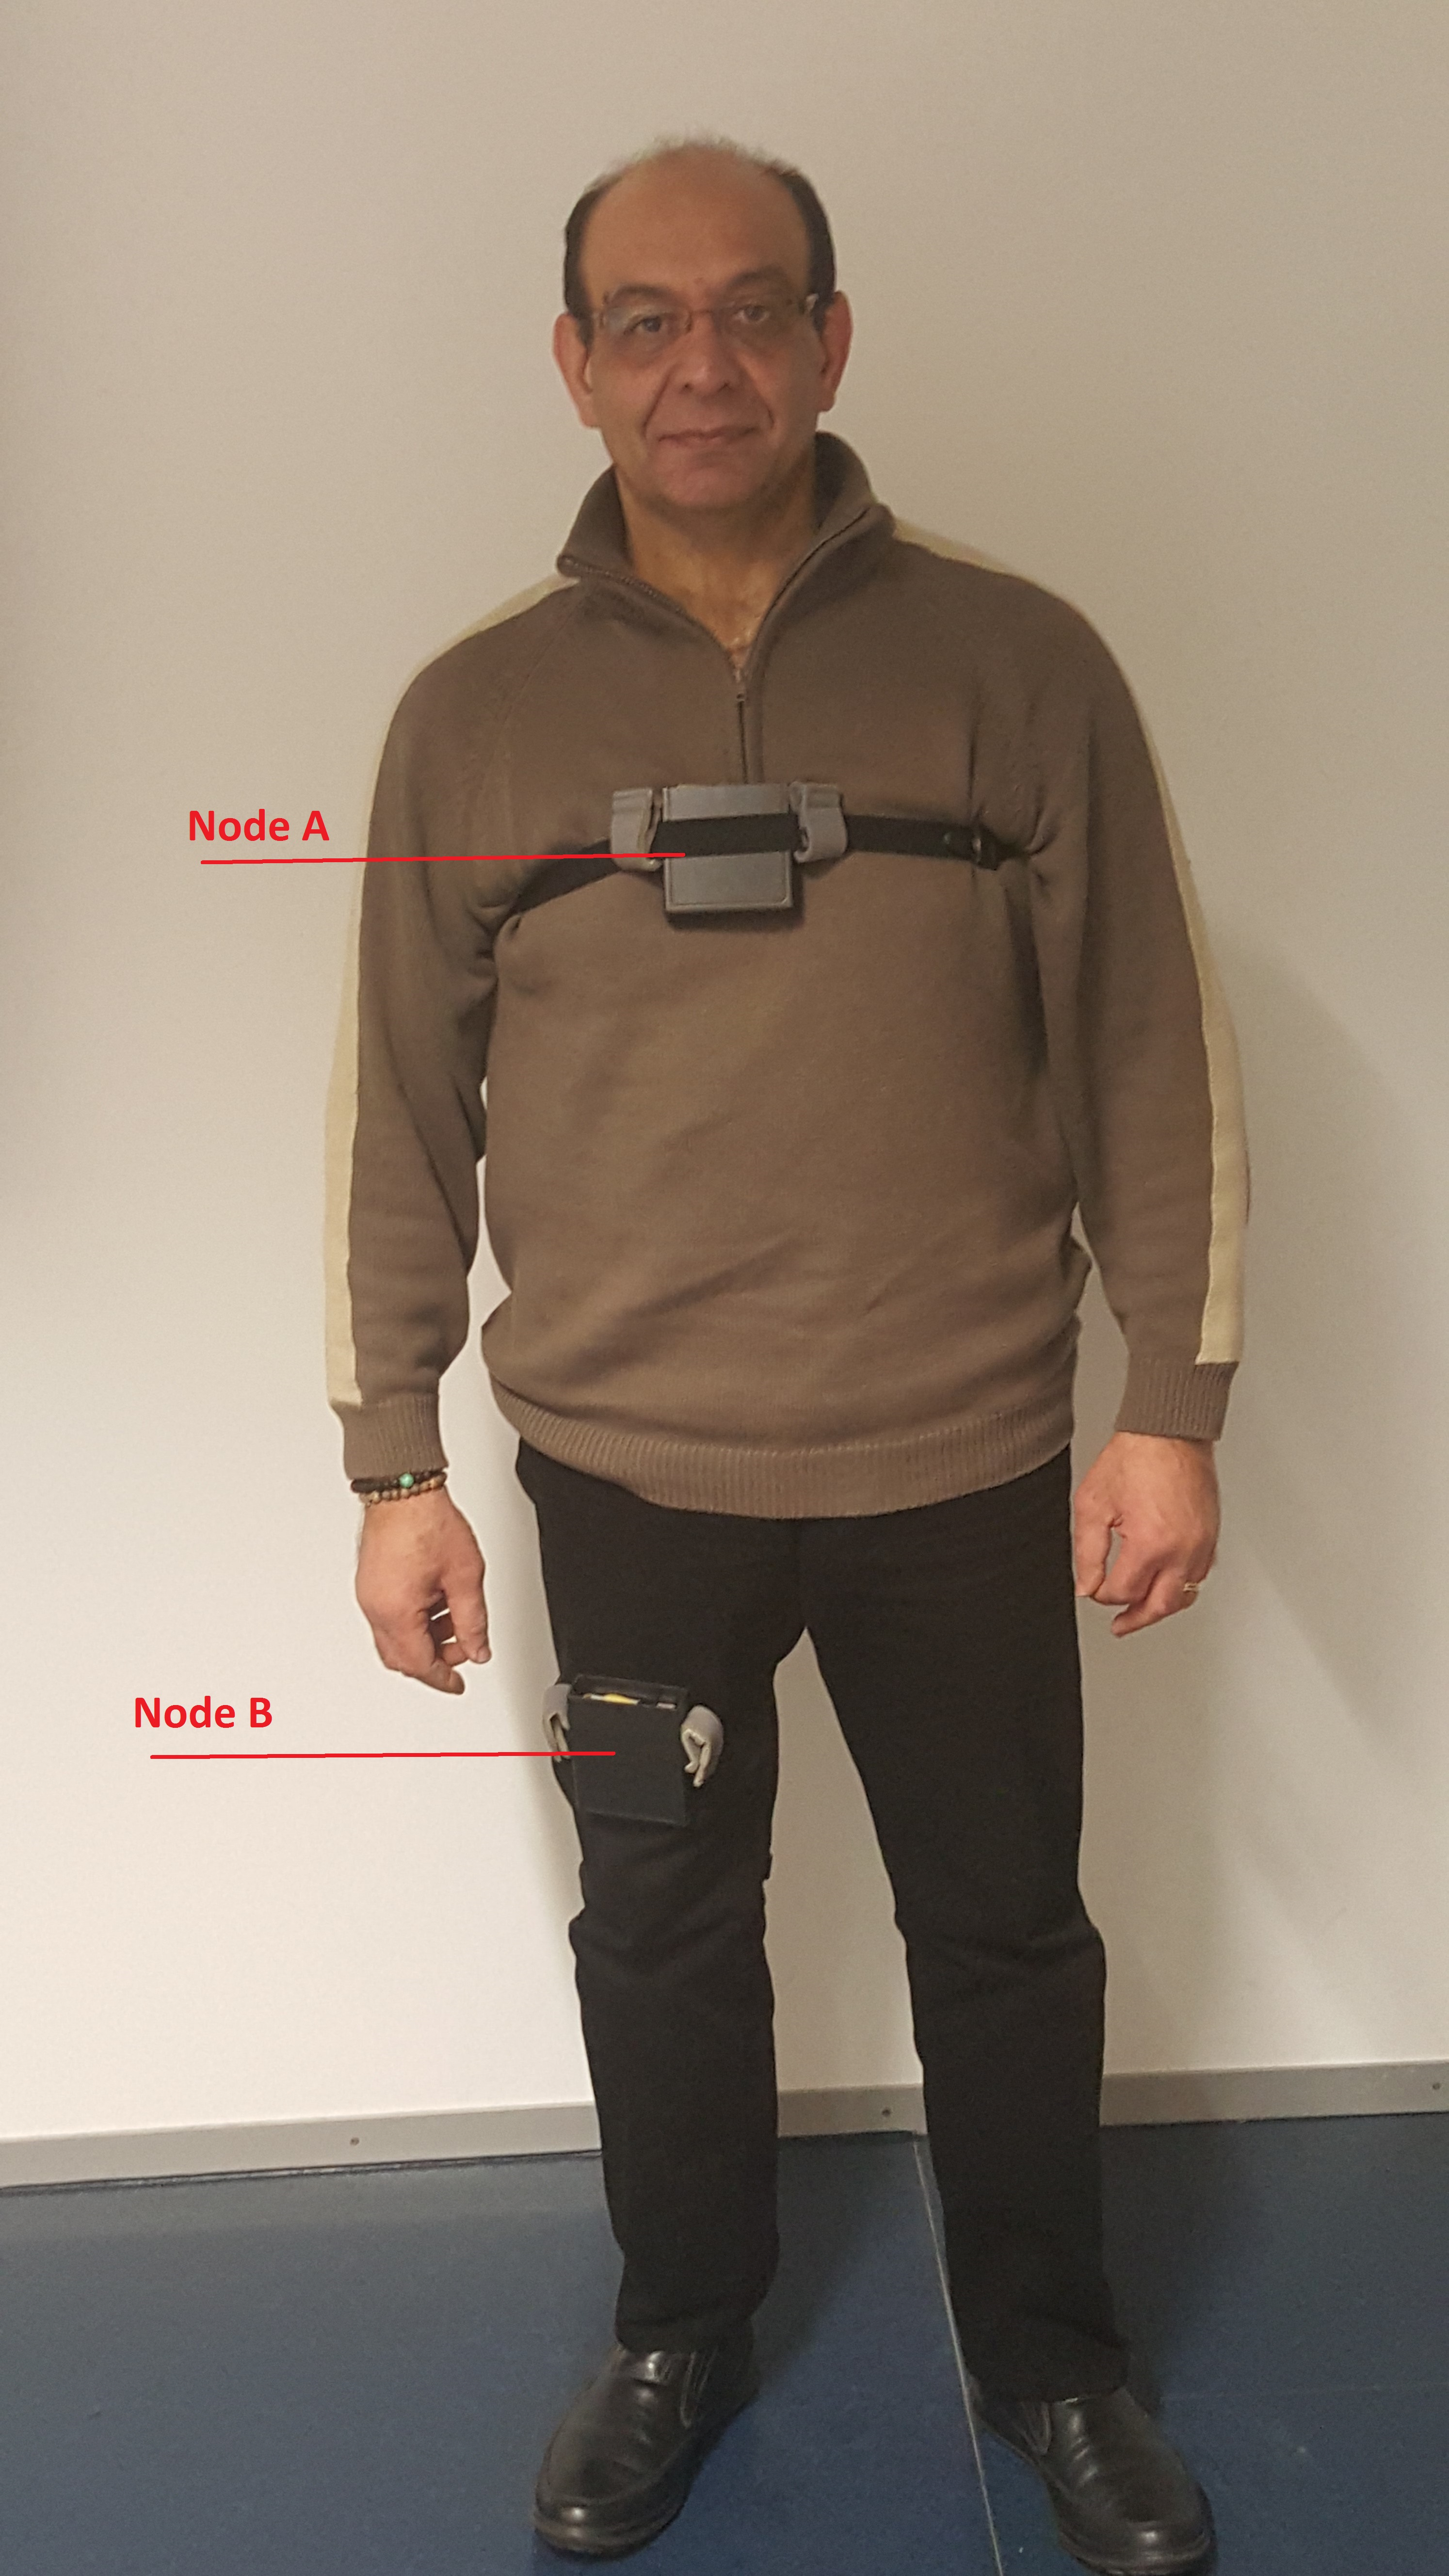
\includegraphics[scale=0.06]{Images/Stankovic_papa2}
	\caption[System architecture according to Li et al.]{System architecture according to Li et al. \cite{Li2009}}
	\label{fig:LietAl-Architecture}
\end{figure}
Li et al. distinguish between two different motion sequences which are used for activity categorization:
\begin{itemize}
	\item Static postures:
	\begin{itemize}
		\item Standing, sitting, lying
	\end{itemize}
	\item Dynamic postures:
	\begin{itemize}
		\item Activities of daily life (ADL) $\rightarrow$ walking, go up / down stairs, sit, jump, lay down, run
		\item Fall-like motions $\rightarrow$ quick sit-down upright, quick sit-down reclined
		\item Flat surface falls $\rightarrow$ fall forward, fall backward, fall right, fall left
		\item Inclined falls $\rightarrow$ fall on stairs
	\end{itemize}
\end{itemize}
A 3-phase Algorithm for fall-detection is proposed by Li et al. to decrease the computational effort of the micro controller. The first phase of the fall-detection algorithm examines if the person is in a static or dynamic position. If the analyzed position coincides with a static postures in the second phase it will be checked whether it corresponds to lying. If lying position, it will be checked if the transition to this posture was intentional or unintentional (3.Phase). To determine it, the previous 5 seconds of data is used. In the case it was unintentional the event will be classified as a fall. The proposed approach in \cite{Li2009} uses a threshold based technique that is applied in the different phases of the algorithm. The weakness of this approach is to differentiate between jumping into bed and falling against wall with seated posture. Collado Villaverde et al. \cite{colladomachine} propose a wearable fall-detection solution based on a smartwatch using acceleration data in combination with machine learning techniques.

A different approach to detect fall-events is presented by Lüder et al. \cite{Luder2009} which apply an air pressure sensor in addition to the accelerometer. The minor air pressure changes correspond to an altitude change of 25 cm which is a relevant indication in combination with accelerometer data of a possible fall-event.  This sensor combination is incorporated in the hardware "StairMaster" of the Frauenhofer Institute. The hardware architecture proposed in \cite{Luder2009} depicts a wearable solution which is worn on the hip and provides wireless data transmission via Bluetooth. Alternatively, the data can be stored on a Secure Digital (SD) card for evaluation purposes. Due to the fact that air pressure can be influenced by meteorological disturbances Lüder et al. \cite{Luder2009} introduced an alternative architecture. This alternative approach incorporates an external barometric sensor as a reference, which is placed in a stationary altitude to compare both air pressure data (wearable \& stationary). Another method for fall-detection based on sensor fusion techniques is described by Gjoreski et al. \cite{Gjoreski2014}. Accelerometer and electrocardiogram (ECG) data is used to detect fall-events. The solution in \cite{Gjoreski2014} is capable of identifying person's movements and fall-situations using wearable sensor nodes based on Bluetooth. These nodes are placed on the chest and thigh which is similar to Li et al's \cite{Li2009} approach. The advantage of the proposed solution by Gjoreski et al. \cite{Gjoreski2014} is the integration of medical sensors. The fusion of acceleration data and ECG-Signal facilitates the detection of anomalies in person's behavior and heart related problems that my lead to falls. The results presented in \cite{Gjoreski2014} emphasize that the incorporation of the ECG-signal can significantly increase the system's reliability to detect fall-events. According to the analysis of Gjoreski et al. \cite{Gjoreski2014} differences in the ECG-signal in different postures were detected. Lower beat rates in the static positions lying and sitting compared to waling were determined. Comparing the beat rates of both static postures (lying and sitting) differences were observed, where the beat rate of lying is lower than the one of sitting.



\section{Background}
\label{sec:background}
The fall-detection prototype is based on the approach proposed in \cite{Gjoreski2014, Kozina}. To detect a fall-event a typical physical behavior is used which comprises the following the phases (see Figure \ref{fig:fallKozina}):
\begin{itemize}
	\item Pre-fall-phase 
	\item Falling phase
	\item Impact phase
	\item Post-fall phase
\end{itemize}
The pre-fall phase illustrates a stationary position of the person where the measured acceleration is around 1g (9.81$m/s^{2}$). During the falling phase the  acceleration decreases close to 0g (0$m/s^{2}$), which depicts a similar behavior to a free fall. Upon the impact (impact phase), the acceleration reaches his maximum value for a short period of time. This signalizes that the person has suffered an impact. Subsequently, the acceleration is decreasing to around 1g (9.81$m/s^{2}$) which represents the post-fall phase because after a fall the person is lying down. To apply this fall-detection pattern the accelerometer data of the sensor nodes is used. Important to know is that for the impact detection the acceleration magnitude is used which is calculated with the following formula ~\ref{eq:acel} and to determine the body's orientation the single axis values of the accelerometer ($\alpha_x$, $\alpha_y$, $\alpha_z$) are analyzed:

\begin{equation}\label{eq:acel}
\alpha = \sqrt{\alpha_{x}^{2} + \alpha_{y}^{2} + \alpha_{z}^{2}}
\end{equation}

\begin{figure}[!ht]
	\centering
	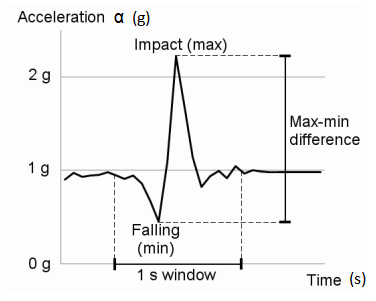
\includegraphics[scale=1]{images/KozinaImpact}
	\caption[Acceleration during impact]{Acceleration during impact according to Kozina et al. ~\cite{Kozina}}
	\label{fig:fallKozina}
\end{figure}
Taking into consideration the body orientation the single acceleration axis ($\alpha_x$, $\alpha_y$, $\alpha_z$) are essential to determine the person's body orientation. Assuming that the person is in a standing position (static posture), the x-acceleration ($\alpha_x$) corresponds to 1g (9.81$m/s^{2}$) and the other two axis ($\alpha_y$, $\alpha_z$) would be close to 0g (0$m/s^{2}$). This is a reference for a standing position. As soon as the person changes his posture, the gravitational force will act on one of the other two axis ($\alpha_y$, $\alpha_z$) and the x-acceleration will be 0g (0$m/s^{2}$). Combining this information with the acceleration magnitude (see Equation \ref{eq:acel}) the system is able to detect the fall and additionally determine the type of fall.

here pannurat and li et al test fall types
\section{Fall-detection system prototype}
\label{sec:fall-detectionPrototype}	

\subsection{Architecture}


\subsection{Sensor fusion}
ECG

\subsection{Generation of test-events}
Lorena's part

\subsection{Detected problems}

\section{Example application of STAMP as hazard analysis method}
\label{sec:STAMP}

\subsection{Introducing STAMP}

\subsection{STAMP - Hazard analysis}

\section{Conclusion \& Future work}
\label{sec:conclusion}

\section{Bibliography styles}

There are various bibliography styles available. You can select the style of your choice in the preamble of this document. These styles are Elsevier styles based on standard styles like Harvard and Vancouver. Please use Bib\TeX\ to generate your bibliography and include DOIs whenever available.

Here are two sample references: \cite{Feynman1963118,Dirac1953888}.

\section*{References}

\bibliography{mybibfile}

\end{document}